


\documentclass{article}
\usepackage[
        a4paper,% other options: a3paper, a5paper, etc
        left=3cm,
        right=3cm,
        top=3cm,
        bottom=4cm,
        % use vmargin=2cm to make vertical margins equal to 2cm.
        % us  hmargin=3cm to make horizontal margins equal to 3cm.
        % use margin=3cm to make all margins  equal to 3cm.
]{geometry}
%\usepackage[utf8x]{inputenc}
\usepackage{graphicx}
\usepackage{caption}
\usepackage{enumerate}
\usepackage{subcaption}
\usepackage[procnames]{listings}
\usepackage{color}
\usepackage{amssymb}
\usepackage{amsmath}
\usepackage{comment}
\usepackage{hyperref}
\usepackage{blindtext}
\usepackage[titletoc,title]{appendix}
\usepackage{float}
\usepackage{fullpage}
\definecolor{codegreen}{rgb}{0,0.6,0}
\definecolor{codegray}{rgb}{0.5,0.5,0.5}
\definecolor{codepurple}{rgb}{0.58,0,0.82}
\definecolor{backcolour}{rgb}{0.95,0.95,0.92}

\lstdefinestyle{mystyle}{
    backgroundcolor=\color{backcolour},
    commentstyle=\color{codegreen},
    keywordstyle=\color{magenta},
    numberstyle=\tiny\color{codegray},
    stringstyle=\color{codepurple},
    basicstyle=\ttfamily,
    breakatwhitespace=false,
    breaklines=true,
    captionpos=t,
    keepspaces=true,
    numbers=left,
    numbersep=5pt,
    showspaces=false,
    showstringspaces=false,
    showtabs=false,
    tabsize=2
}

\lstset{style=mystyle, language=Matlab}

\renewcommand{\thesection}{\large{Exercise \arabic{section}}}

\title{Computer Vision - Lab 3}
\author{Luuk Boulogne (s2366681) \and Steven Bosch (s1861948)}
\date{\today}

\begin{document}
\maketitle

\begin{figure}[ht!]
 \centering
 \begin{subfigure}{.3\textwidth}
  \centering
  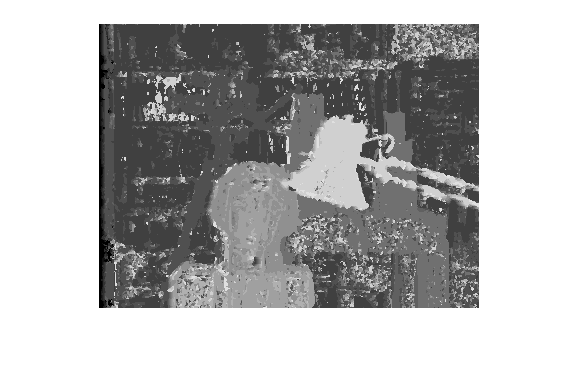
\includegraphics[width=\linewidth]{ex3/a5_5g.png}
  \caption{$5\times5$ gaussian window}
  \label{fig_a1}
 \end{subfigure}
 \begin{subfigure}{.3\textwidth}
  \centering
  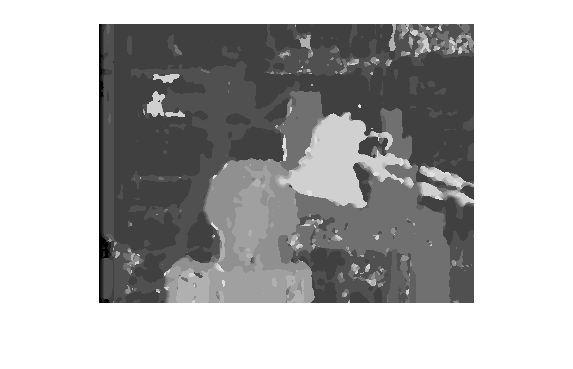
\includegraphics[width=\linewidth]{ex3/a10_10g.png}
  \caption{$10\times10$ gaussian window}
  \label{fig_a2}
 \end{subfigure}
 \begin{subfigure}{.3\textwidth}
  \centering
  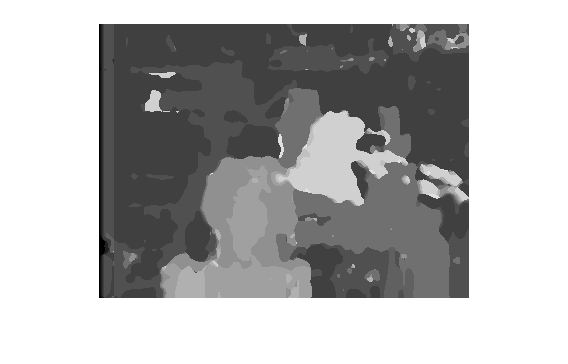
\includegraphics[width=1\linewidth]{ex3/a15_15g.png}
  \caption{$15\times15$ gaussian window}
  \label{fig_a3} 
 \end{subfigure}
 
 \begin{subfigure}{.3\textwidth}
  \centering
  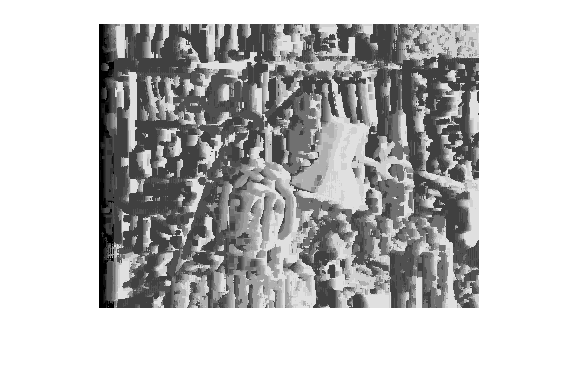
\includegraphics[width=\linewidth]{ex3/a5_5.png}
  \caption{$5\times5$ window}
  \label{fig_a1g}
 \end{subfigure}
 \begin{subfigure}{.3\textwidth}
  \centering
  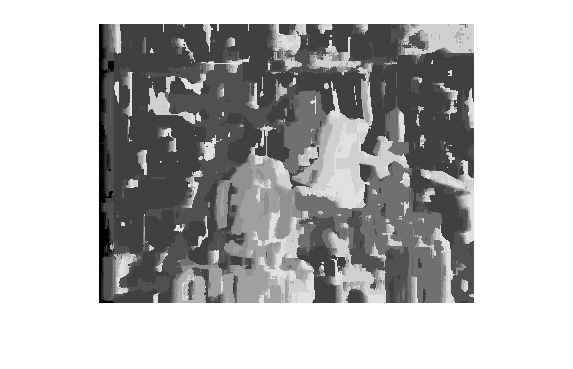
\includegraphics[width=\linewidth]{ex3/a10_10.png}
  \caption{$10\times10$ window}
  \label{fig_a2g}
 \end{subfigure}
 \begin{subfigure}{.3\textwidth}
  \centering
  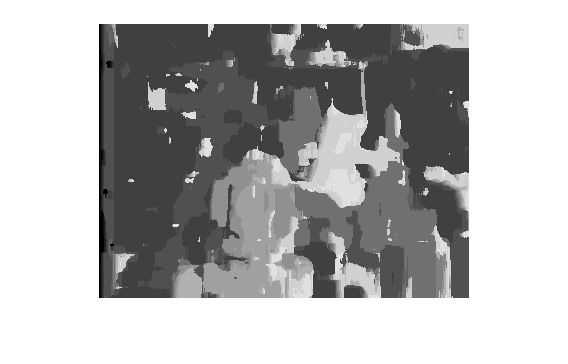
\includegraphics[width=1\linewidth]{ex3/a15_15.png}
  \caption{$15\times15$ window}
  \label{fig_a3g}
 \end{subfigure}
 \caption{Depth maps constructed using the absolute difference as difference measure with varied window size and shape.}
 \label{fig_a}
\end{figure}

\begin{figure}[ht!]
 \centering
 \begin{subfigure}{.3\textwidth}
  \centering
  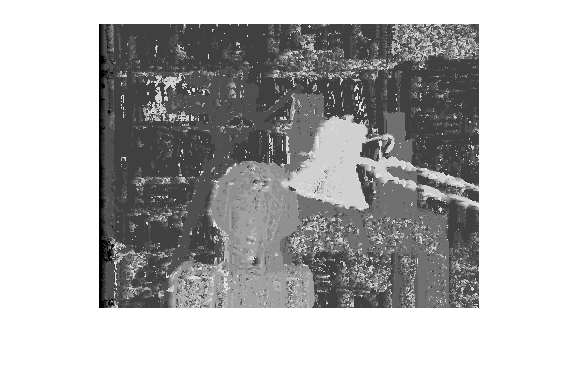
\includegraphics[width=\linewidth]{ex3/s5_5g.png}
  \caption{$5\times5$ gaussian window}
  \label{fig_s1}
 \end{subfigure}
 \begin{subfigure}{.3\textwidth}
  \centering
  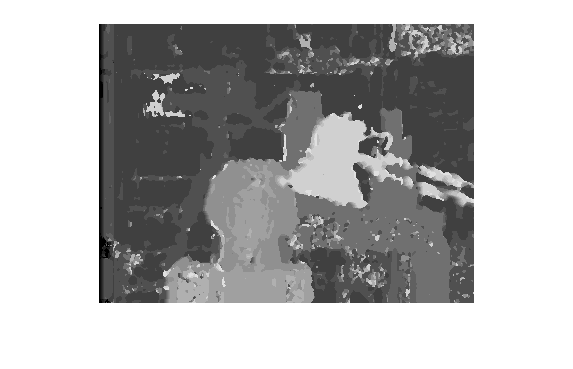
\includegraphics[width=\linewidth]{ex3/s10_10g.png}
  \caption{$10\times10$ gaussian window}
  \label{fig_s2}
 \end{subfigure}
 \begin{subfigure}{.3\textwidth}
  \centering
  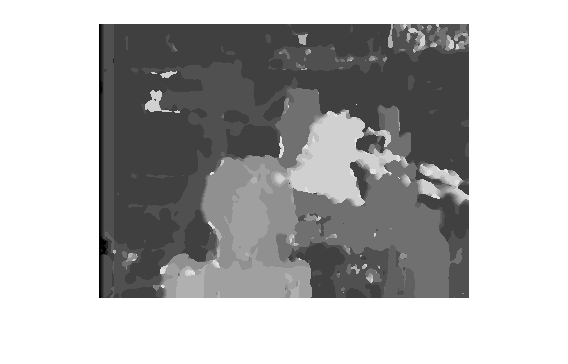
\includegraphics[width=1\linewidth]{ex3/s15_15g.png}
  \caption{$15\times15$ gaussian window}
  \label{fig_s3} 
 \end{subfigure}
 
 \begin{subfigure}{.3\textwidth}
  \centering
  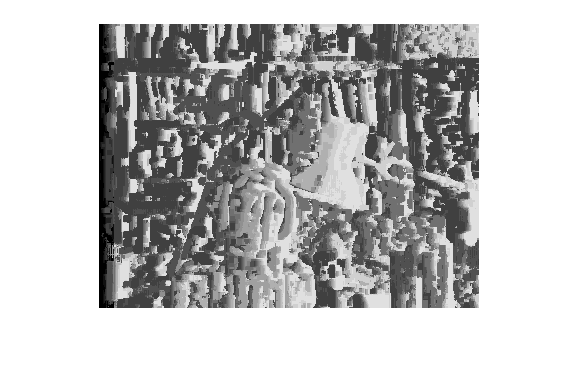
\includegraphics[width=\linewidth]{ex3/s5_5.png}
  \caption{$5\times5$ window}
  \label{fig_s1g}
 \end{subfigure}
 \begin{subfigure}{.3\textwidth}
  \centering
  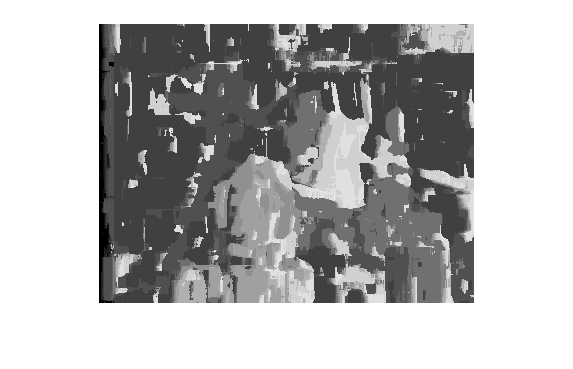
\includegraphics[width=\linewidth]{ex3/s10_10.png}
  \caption{$10\times10$ window}
  \label{fig_s2g}
 \end{subfigure}
 \begin{subfigure}{.3\textwidth}
  \centering
  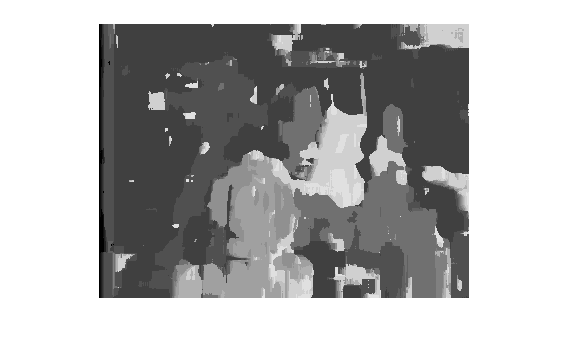
\includegraphics[width=1\linewidth]{ex3/s15_15.png}
  \caption{$15\times15$ window}
  \label{fig_s3g}
 \end{subfigure}
 \caption{Depth maps constructed using the squared difference as difference measure with varied window size and shape.}
 \label{fig_s}
\end{figure}



\begin{figure}[ht!]
 \centering
 \begin{subfigure}{.3\textwidth}
  \centering
  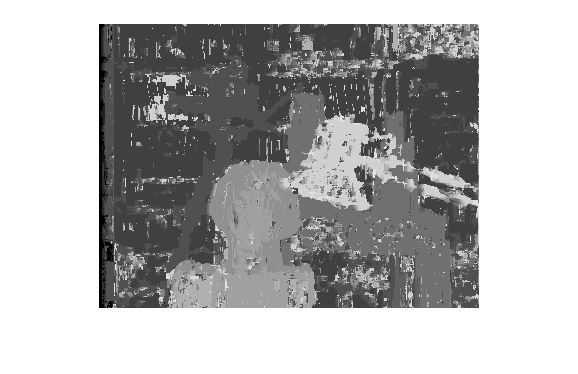
\includegraphics[width=\linewidth]{ex3/x5_5.png}
  \caption{$5\times5$ window}
  \label{fig_x1g}
 \end{subfigure}
 \begin{subfigure}{.3\textwidth}
  \centering
  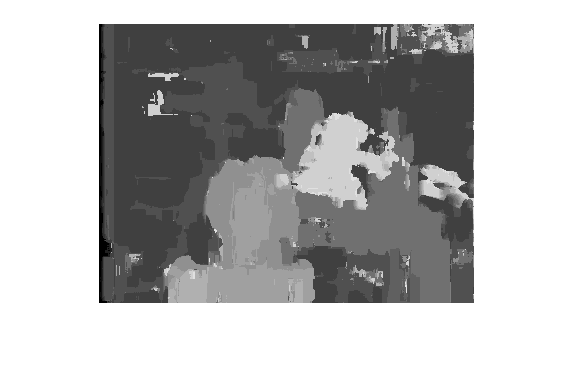
\includegraphics[width=\linewidth]{ex3/x10_10.png}
  \caption{$10\times10$ window}
  \label{fig_x2g}
 \end{subfigure}
 \begin{subfigure}{.3\textwidth}
  \centering
  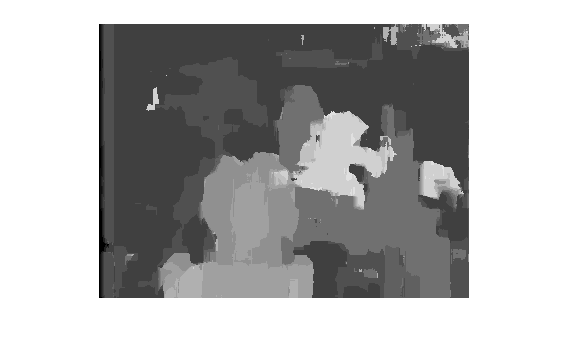
\includegraphics[width=1\linewidth]{ex3/x15_15.png}
  \caption{$15\times15$ window}
  \label{fig_x3g}
 \end{subfigure}
 \caption{Depth maps constructed using the normalized cross correlation as similarity measure with varied window size.}
 \label{fig_x}
\end{figure}



\section{}
The window sizes we compared are $5\times5$, $10\times10$ and $15\times15$. For the absolute difference and squared difference functions, we also changed the shape of the window by multiplying the compared patches with a 2D gaussian window. We compared the results of this with the results when the gaussian window has not been applied. All results are shown in figures \ref{fig_a}, \ref{fig_s} and \ref{fig_x}.

For all window sizes and shapes, the absolute and s

\end{document}